\documentclass[hidelinks,12pt,a4paper]{article}
\usepackage[italian]{babel}
\usepackage[utf8]{inputenc}
\usepackage{fourier} 

% Images
\usepackage{graphicx}
\usepackage{caption}
\usepackage{subcaption}
\usepackage{float}
\graphicspath{ {../Decolorized_Images} }

% Stop hyphenation
\usepackage[none]{hyphenat}

% Adjust paragraph.
\usepackage{changepage}

% License
\usepackage[
type={CC},
modifier={by-nc-sa},
version={4.0},
]{doclicense}

\begin{document}
	
	\title{\textbf{\centering{Laboratorio creativo per bambini}\\Colora le opere d'arte}}
	\author{Alice Balestieri}
	\date{}
	
	\maketitle
	\newpage
	
	\tableofcontents
	\newpage
	
	\section{Come giocare}
	\begin{center}
		\textbf{Le regole sono rivolte agli operatori.}
	\end{center}
	
	Far divertire i bambini a colorare le immagini delle opere decolorate.
	
	\newpage
	\section{Immagini}
		\begin{adjustwidth}{-30mm}{-30mm}
			\bigskip
			
			\begin{minipage}{\linewidth}
				\centering
				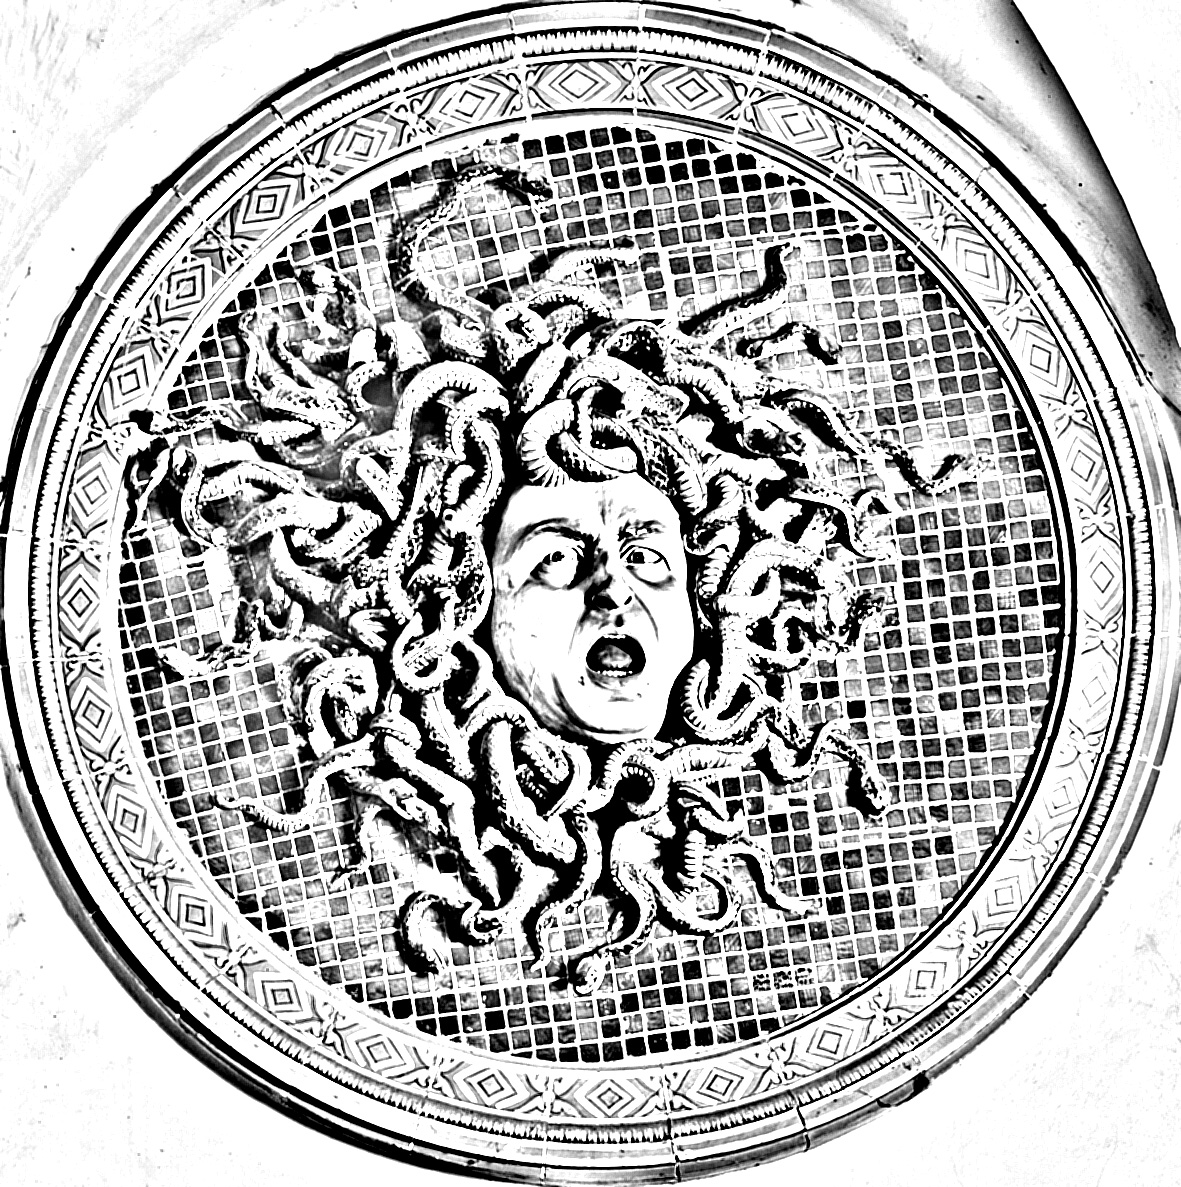
\includegraphics[scale=2]{Mengaroni_Ferruccio-Medusa.jpg}
			\end{minipage}
			
			\vspace*{\fill}
			\fboxrule=4pt{
					\fbox
				{
					\begin{minipage}[t][55pt][t]{0.91\linewidth}
					Mengaroni Ferruccio - Medusa - Colorata da: 
					\end{minipage}
				}
				}
			
		\end{adjustwidth}
\end{document}